\section{Hartree-Fock calculation of asymmetric nuclear matter}%
\label{sec:hartree_fock_calculation_of_asymmetric_nuclear_matter}

In this section, we only limit ourselves to two-body interaction, thus, the nucleon-nucleon (\gls{NN}) potential can be expressed in the form of
\begin{equation}
        v = v(\bm{r}, \bm{r'}, \bm{p}, \bm{p'}, \bm{\sigma}, \bm{\sigma'}, \bm{\tau}, \bm{\tau'})
        \label{eff_interaction}
\end{equation}
where the primed and unprimed variables indicate the properties of 2 nucleons respectively, in which $\bm{r}$ is the particle's position, $\bm{p}$ is its momentum, $\bm{\sigma}$ is its intrinsic spin and $\bm{\tau}$ is its isospin.\par
The functional form of $v$ in \eqref{eff_interaction} cannot freely take any form but is constrained by many invariance requirements \citep{greiner1996nuclear}, namely the translational, Galilei, rotational, isospin, parity and time reversal invariance. Having such considerations, the central component of \gls{NN} interaction potential is expressed as function of the distance $r$ between interacting nucleons
\begin{equation}
        v = v_{00}(r) + v_{10}(r) \bm{\sigma}\cdot\bm{\sigma'} + v_{01}(r) \bm{\tau}\cdot\bm{\tau'} + v_{11}(r) (\bm{\sigma}\cdot\bm{\sigma'})(\bm{\tau}\cdot\bm{\tau'})
\end{equation}
There exists another composition of the interaction, i.e. the \emph{spin-orbit} terms, however, as stated by \cite{vidana2016role}, their contributions are much smaller than the central one, and have yet to be included in the present study. Due to the lack of an exact theory to describe the \gls{NN} interaction, a model needs to be imposed and fit with experimental measurement or theoretical calculation results. Furthermore, for a system as massive as a \gls{NS}, deducing the \gls{EoS} of the matter using the \emph{ab initio} method, i.e. solving the Schr\"{o}dinger equation over all particles, is impossible; therefore an \emph{effective interaction} must be used \citep{greiner1996nuclear}. Here, among various interaction models, the CDM3Y$n$ interaction was chosen. This interaction is constructed based on the M3Y-Paris interaction, which was used successfully in the \gls{HF} study of \gls{NM} \citep{loan2011equation, tan2016mean, tan2020spin,tan2021equation} and the folding model study of \gls{NN} scattering \citep{khoa1997nuclear,khoa2000generalized}, with the direct (exchange) central terms being expressed as
\begin{equation}
    v^{D(EX)} = v^{D(EX)}_{00}(r) + v^{D(EX)}_{10}(r) \bm{\sigma}\cdot\bm{\sigma'} + v^{D(EX)}_{01}(r) \bm{\tau}\cdot\bm{\tau'} + v^{D(EX)}_{11}(r) (\bm{\sigma}\cdot\bm{\sigma'})(\bm{\tau}\cdot\bm{\tau'})
\end{equation}
The density-dependence of the \gls{NN} interaction is encoded into an additional form factor $F_{\sigma\tau}(n_b)$ multplied to each $\sigma\tau$-term, which gives rise to the explicit form of the CDM3Y$n$ interactions, i.e.
\begin{IEEEeqnarray*}{rCl}
        v^{D(EX)}(n_b,r) &=& F_{00}(n_b) v^{D(EX)}_{00}(r) + F_{10}(n_b) v^{D(EX)}_{10}(r) \bm{\sigma}\cdot\bm{\sigma'}\\
                          &&\negmedspace{}+ F_{01}(n_b) v^{D(EX)}_{01}(r) \bm{\tau}\cdot\bm{\tau'} + F_{11}(n_b) v^{D(EX)}_{11}(r) (\bm{\sigma}\cdot\bm{\sigma'})(\bm{\tau}\cdot\bm{\tau'})\IEEEyesnumber
                          \label{eqHF}
\end{IEEEeqnarray*}
where each radial term is the superposition of 3 Yukawa potentials
\begin{equation}
    v^{D(EX)}_{\sigma\tau}(r) = \sum^{3}_{k=1} Y^{D(EX)}_{\sigma\tau}(k) \frac{\exp(-\mu_k r)}{\mu_k r} 
\end{equation}
with the Yukawa strengths given in Table \ref{tab:yukawa}. The form factors $F_{\sigma\tau}(n_b)$ shared the functional form \citep{khoa1997nuclear,tan2020spin,tan2021equation,than2010ufr}
\begin{equation}
        F_{\sigma\tau}(n) = C_{\sigma\tau} [1 + \alpha_{\sigma\tau} \exp(-\beta_{\sigma\tau}n) + \gamma_{\sigma\tau}n]
\end{equation}
with parameters given in Table \ref{tab:cd}. The parameters of $F_{00}$ were adjusted to give the corresponding values of incompressibility $K$ of symmetric \gls{NM} at saturation density $n_0$ and the binding energy $E_0 \approx 15.8\; MeV$, while the 10 term is modified from \citep{than2010ufr} to reproduce $E_{sym}(n_0) \approx 30\;MeV$, $L\approx 50\;MeV$ and to be in agreement with the ab-initio results \citep{akmal1998equation,gandolfi2010microscopic} at higher density \citep{tan2021equation}.
\begin{table}[H]
        \centering
        \caption{Yukawa strengths of the M3Y-Paris interaction \citep{tan2020spin,anantaraman1983effective}.}
        \label{tab:yukawa}
        \begin{tabular}{|C|C|C|C|C|C|}
                \hline
                k & \mu_k & Y^D_{00} & Y^D_{10} & Y^D_{01} & Y^D_{11}\\
                    & (fm^{-1}) & (MeV) & (MeV) & (MeV) & (MeV)\\
                \hline
                1 & 4.0& 11061.625 & 938.875 & 313.625 & -969.125\\
                2 & 2.5 & -2537.5 & -36.0 & 223.5 & 450.0 \\
                3 & 0.7072 & 0.0 & 0.0 & 0.0 & 3.4877\\
                \hline\hline
                k & \mu_k & Y^{EX}_{00} & Y^{EX}_{10} & Y^{EX}_{01} & Y^{EX}_{11}\\
                    & (fm^{-1}) & (MeV) & (MeV) & (MeV) & (MeV)\\
                \hline
                1 & 4.0 & -1524.25 & -3492.75 & -4118.0 & -2210.0\\
                2 & 2.5 & -518.75 & 795.25 & 1054.75 & 568.75\\
                3 & 0.7072 & -7.8474 & 2.6157 & 2.6157 & -0.8719\\
                \hline
        \end{tabular}
\end{table}
\begin{table}[ht]
        \centering
        \caption{CDM3Y$n$ interaction's parameters; the 00 and 01 terms are inherited from \citep{tan2021equation}, while the 10 and 11 parameters are added by fitting with \gls{BHF} result and $K$ is the incompressibility \eqref{eq:K} of spin-saturated symmetric \gls{NM} at saturation density $n_0\approx 0.17\:fm^{-3}$.}
        \label{tab:cd}
        \begin{tabular}{|C|C|C|C|C|C|C|}
                \hline
                \text{Interaction} & \sigma\tau & C_{\sigma\tau} & \alpha_{\sigma\tau} & \beta_{\sigma\tau} & \gamma_{\sigma\tau} & K\\
                                   & & & & (fm^3) & (fm^3) & (MeV)\\
                \hline
                % \multirow{4}{*}{\text{CDM3Y3}} & 00 & 0.2985 & 3.4528 & 2.6388 & -1.5 &\multirow{4}{*}{217}\\
                %                                & 01 & 0.2343 & 5.3336 & 6.4738 & 4.3172 &\\
                %                                & 10 & 0.3890 & 3.5635 & -2.6717 & 20.3624 &\\
                %                                & 11 & 0.8802 & 4.0433 & 12.3262 & 0.3662 &\\
                % \hline
                \multirow{4}{*}{\text{CDM3Y4}} & 00 & 0.3052 & 3.2998 & 2.3180 & -2.0 &\multirow{4}{*}{228}\\
                                               & 01 & 0.2129 & 6.3581 & 7.0584 & 5.6091 &\\
                                               & 10 & 0.2593 & 6.0016 & -2.3377 & 18.8725 &\\
                                               & 11 & 0.8329 & 3.5941 & 9.2012 & 0.2690 &\\
                \hline
                \multirow{4}{*}{\text{CDM3Y5}} & 00 & 0.2728 & 3.7367 & 1.8294 & -3.0 &\multirow{4}{*}{241}\\
                                               & 01 & 0.2204 & 6.6146 & 7.9910 & 6.0040 &\\
                                               & 10 & 0.4106 & 5.6265 & -1.6698 & -1.9866 &\\
                                               & 11 & 0.6815 & 2.5833 & 5.1700 & 0.2578 &\\
                \hline
                \multirow{4}{*}{\text{CDM3Y6}} & 00 & 0.2658 & 3.8033 & 1.4099 & -4.0 &\multirow{4}{*}{252}\\
                                               & 01 & 0.2313 & 6.6865 & 8.6775 & 6.0182 &\\
                                               & 10 & 0.5186 & 9.9402 & 1.6698 & 2.9799 &\\
                                               & 11 & 0.6058 & 3.1947 & 4.4512 & 0.0822 &\\
                \hline
                \multirow{4}{*}{\text{CDM3Y8}} & 00 & 0.2658 & 3.8033 & 1.4099 & -4.3 &\multirow{4}{*}{257}\\
                                               & 01 & 0.2643 & 6.3836 & 9.8950 & 5.4249 &\\
                                               & 10 & 0.5997 & 9.1900 & 0.7514 & -4.7181 &\\
                                               & 11 & 0.3786 & 3.9435 & 2.7012 & 0.3512 &\\
                \hline
                % \multirow{4}{*}{\text{BDM3Y1}} & 00 & 1.2521 & 0.0 & 0.0 & -1.7452 &\multirow{4}{*}{270}\\
                %                                & 01 & 0.2528 & 7.6996 & 11.0386 & 6.3568 &\\
                %                                & 10 & -1.3226 & -8.2559 & 0.0 & 17.2307 &\\
                %                                & 11 & 0.1654 & 9.7394 & 1.6714 & -1.4893 &\\
                % \hline
        \end{tabular}
\end{table}

On the other hand, in Table \ref{tab:cd}, the spin-dependent terms (10 and 11) are hereby included in 4 models by fine tuning the parameters to yield close result to the Brueckner-Hartree-Fock (\gls{BHF}) study of spin polarized \gls{NM} by \cite{vidana2002equation} as in Figure \ref{fig:bhf}.
\begin{figure}[ht]
        \centering
        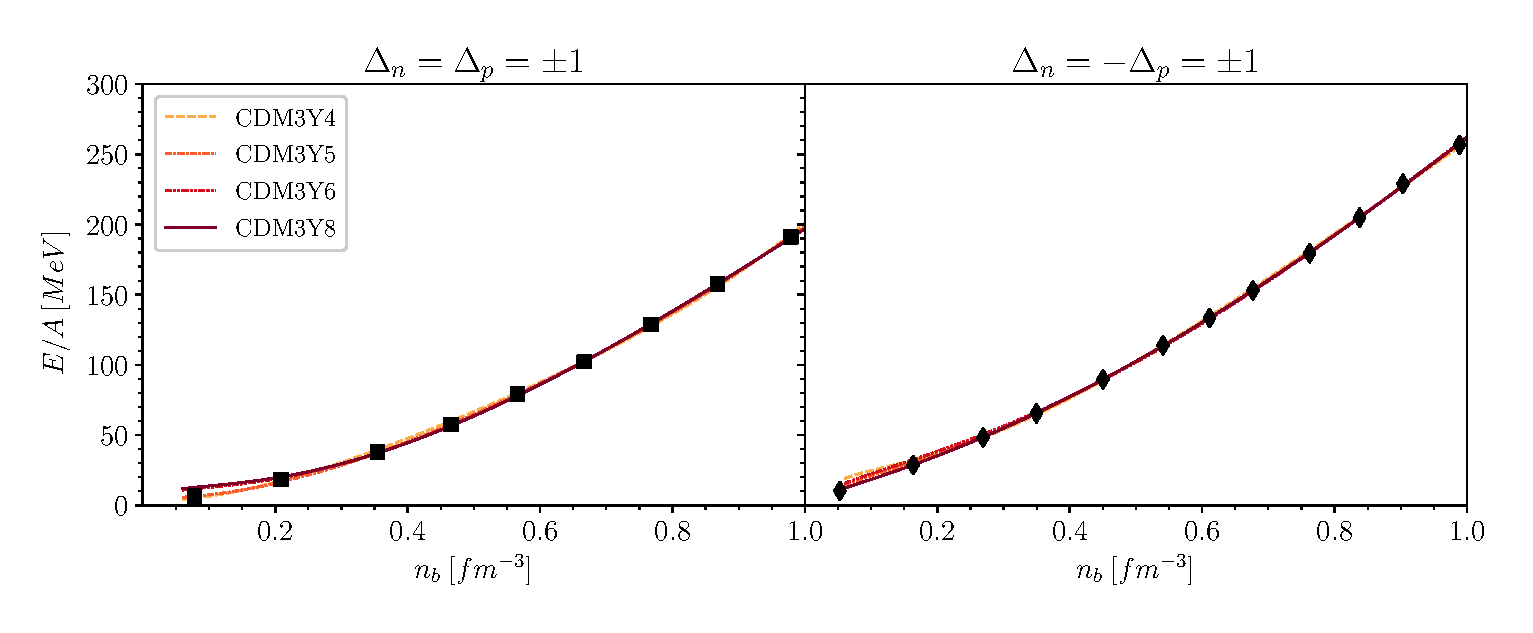
\includegraphics[width=\textwidth]{fig/BHF_fit.eps}
        \caption{Energy per baryon $E/A$ of symmetric \gls{NM} by the 4 CDM3Y$n$ models compared to \gls{BHF} result \citep{vidana2002equation}. The diamond and square represent the \gls{BHF} result for $\Delta_n=-\Delta_p=\pm 1$ and $\Delta_n=\Delta_p=\pm 1$ respectively with $\Delta_\tau$ being the baryon spin polarization.}
        \label{fig:bhf}
\end{figure} 

In \gls{HF} formalism, the total \gls{HF} energy of the system can be expressed as
\begin{IEEEeqnarray*}{rCl}
        E_{HF} &=& \sum^{}_{\sigma\tau} \sum^{k_F^{\sigma\tau}}_{\bm{k}} \frac{\hbar^2 k^2}{2m_\tau} + \frac{1}{2} \sum^{}_{\bm{k}\sigma\tau} \sum^{}_{\bm{k'}\sigma'\tau'} \left[ \mel**{\bm{k}\sigma\tau,\bm{k'}\sigma'\tau'}{v^D}{\bm{k}\sigma\tau,\bm{k'}\sigma'\tau'} \right.\\
          && \left. \negmedspace{} + \mel**{\bm{k}\sigma\tau,\bm{k'}\sigma'\tau'}{v^{EX}}{\bm{k'}\sigma\tau,\bm{k}\sigma'\tau'} \right]\IEEEyesnumber
          \label{eqE}
\end{IEEEeqnarray*}  
with $\Omega$ being the spatial volume of the system, $k_F^{\sigma\tau} = (6\pi^2 n_{\sigma\tau})^{1/3}$ is the Fermi momentum corresponding to spin $\sigma$ and isospin $\tau$, the first double summation is the \emph{kinetic energy} of the system, while the other being its \emph{potential energy}.

Dividing \eqref{eqE} by the system total volume $\Omega$, the energy density of the \gls{NM} is separated into the kinetic term $\varepsilon_{kin}$ and the potential terms $\varepsilon_{\sigma\tau}$, i.e.
\begin{equation}
        \varepsilon_{HF} = \frac{E_{HF}}{\Omega} = \varepsilon_{kin} + F_{00}(n_b) \varepsilon_{00} + F_{01}(n_b) \varepsilon_{01} + F_{10}(n_b) \varepsilon_{10} + F_{11}(n_b) \varepsilon_{11}
\end{equation}
The final expressions of each terms of the energy density are
{\allowdisplaybreaks
\begin{IEEEeqnarray}{rCl}
        \varepsilon_{kin} &=& \frac{3}{10} \sum^{}_{\sigma\tau} \frac{\hbar^2 (k_F^{\sigma\tau})^2}{m_\tau} n_{\sigma\tau}\\
        \varepsilon_{00} &=& \frac{1}{2} \left[ n_b^2 J^D_{00} + \int {A^2_{00} v^{EX}_{00}(r)} \: d^3 r \right] \\
        \varepsilon_{10} &=& \frac{1}{2} \left[ n_b^2 J^D_{10} \left( \Delta_n \frac{1+\delta}{2} + \Delta_p \frac{1-\delta}{2} \right)^2 + \int {A^2_{10} v^{EX}_{10}(r)} \: d^3 r \right] \\
        \varepsilon_{01} &=& \frac{1}{2} \left[ n_b^2 J^D_{01}\delta^2 + \int {A^2_{01} v^{EX}_{01}(r)} \: d^3 r \right] \\
        \varepsilon_{11} &=& \frac{1}{2} \left[ n_b^2 J^D_{11} \left( \Delta_n \frac{1+\delta}{2} - \Delta_p \frac{1-\delta}{2} \right)^2 + \int {A^2_{11} v^{EX}_{11}(r)} \: d^3 r \right]
\end{IEEEeqnarray}  
}
where $\Delta_{\tau} = (n_{\uparrow \tau} - n_{\downarrow \tau})/n_{\tau}$ is the polarization of nucleon, $\delta = (n_n - n_p)/n_b$ is the asymmetry of \gls{NM}, $J^D_{\sigma\tau} = \int v^D_{\sigma\tau}(r)\: d^3 r$ is the volume integral of the direct interaction and
\begin{equation}
        \begin{array}{l}
                A_{00} = n_{\uparrow n} \hat{j_1}(k_F^{\uparrow n} r) + n_{\downarrow n} \hat{j_1}(k_F^{\downarrow n} r) + n_{\uparrow p} \hat{j_1}(k_F^{\uparrow p} r) + n_{\downarrow p} \hat{j_1}(k_F^{\downarrow p} r)\\[5pt]
                A_{10} = n_{\uparrow n} \hat{j_1}(k_F^{\uparrow n} r) - n_{\downarrow n} \hat{j_1}(k_F^{\downarrow n} r) + n_{\uparrow p} \hat{j_1}(k_F^{\uparrow p} r) - n_{\downarrow p} \hat{j_1}(k_F^{\downarrow p} r)\\[5pt]
                A_{01} = n_{\uparrow n} \hat{j_1}(k_F^{\uparrow n} r) + n_{\downarrow n} \hat{j_1}(k_F^{\downarrow n} r) - n_{\uparrow p} \hat{j_1}(k_F^{\uparrow p} r) - n_{\downarrow p} \hat{j_1}(k_F^{\downarrow p} r)\\[5pt]
                A_{11} = n_{\uparrow n} \hat{j_1}(k_F^{\uparrow n} r) - n_{\downarrow n} \hat{j_1}(k_F^{\downarrow n} r) - n_{\uparrow p} \hat{j_1}(k_F^{\uparrow p} r) + n_{\downarrow p} \hat{j_1}(k_F^{\downarrow p} r)
        \end{array}
\end{equation}
with $\hat{j}_1(x)=3j_1(x)/x$ and $j_1(x)$ being the 1\textsuperscript{st} order spherical Bessel function.

In the parabolic approximation \citep{khoa1996study}, the energy density per nucleon $E/A$ can also be expanded in terms of the asymmetry $\delta$ as
\begin{equation}
    \frac{E}{A} (n_b, \delta, \Delta_n, \Delta_p) = \frac{\varepsilon_{HF}}{n_b} = \frac{E}{A} (n_b, \delta=0, \Delta_n, \Delta_p) + S(n_b, \Delta_n, \Delta_p)\delta^2 + \mathcal{O}(\delta^4)
    \label{eq:S}
\end{equation}
with $S$ being the \emph{nuclear symmetry energy}. The nuclear symmetry energy is well constrained at low baryon density by the study of heavy-ion (\gls{HI}) collisions \citep{tsang2011constraints,ono2003isospin}, the structure study of the giant dipole resonance by \cite{trippa2008giant} or the neutron skin \citep{furnstahl2002neutron}. As shown in Figure \ref{fig:s}, the symmetry energy $S$ \eqref{eq:S} of symmetric ($\delta = 0$) \gls{NM} is calculated for each interaction in different polarizations and compared to the empirical data, along with other nuclear models (\gls{APR} and \gls{MMC}). It's clear that the more strongly \gls{NM} polarizes under magnetic field, the higher the symmetry energy $S$ is. Moreover, at high values of $\Delta$, $S$ falls completely outside of the \gls{HI} range suggested, while the cases of weaker or without polarization appear to remain well within this range, as well as the 90\% \gls{CFL} region of the astrophysical constraint of GW170817 \citep{xie2019bayesian}.\par

\begin{figure}[ht!]
        \centering
        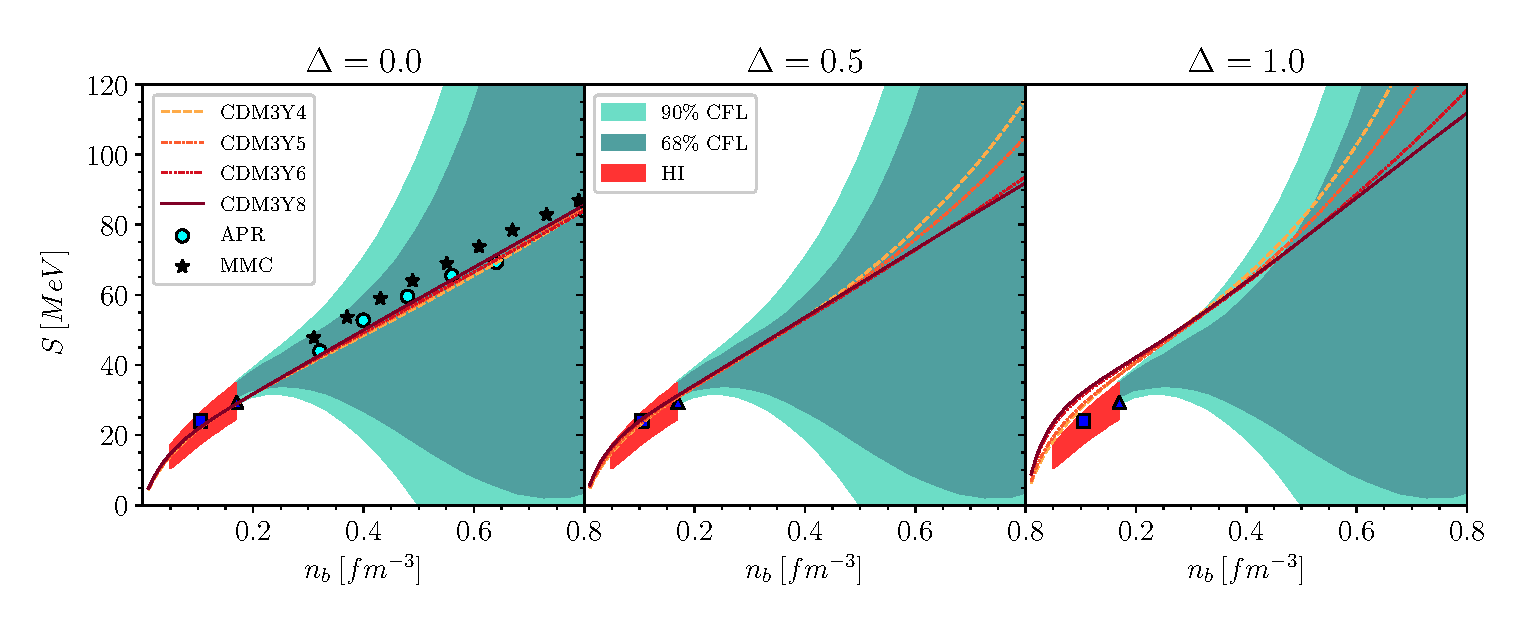
\includegraphics[width=\textwidth]{fig/S.eps}
        \caption{Symmetric energy $S$ of symmetric \gls{NM} at increasing polarization with 4 CDM3Y$n$ interaction models. The shaded areas are the empirical ranges obtained from the Bayesian study \citep{xie2019bayesian} of the \gls{NS} of radius $R_{1.4}$ at 68\% and 90\% confident level (\gls{CFL}) with the GW170817 event \citep{abbott2018gw170817}. The square and triangle are the values suggested by the structure study of \cite{trippa2008giant} and \cite{furnstahl2002neutron}. The circles and stars are the ab-initio result of \cite{akmal1998equation} (\gls{APR}) and microscopic Monte Carlo (\gls{MMC}) calculation by \cite{gandolfi2010microscopic}.}
        \label{fig:s}
\end{figure}

The same conclusion can be drawn from the energy per baryon $E/A$ of symmetric \gls{NM} (Figure \ref{fig:eas}), as it is in good agreement with the \gls{APR} \citep{akmal1998equation} and \gls{MMC} results \citep{gandolfi2010microscopic} at the spin saturated ($\Delta\approx 0$) scenario, similar to the work of \cite{tan2021equation} on an older version of CDM3Y8 interaction. The astrophysical constraint from GW170817, on the other hand, is much narrower than that for the nuclear symmetry energy $S$ and thus well constraints the value of $E/A$ at high baryon density. As $\Delta$ increases from $0.0$ to $1.0$, the energy per baryon rises significantly, which indicates a scenario of spin saturated \gls{NM} for $n_b > n_0$.
\begin{figure}[ht!]
    \centering
    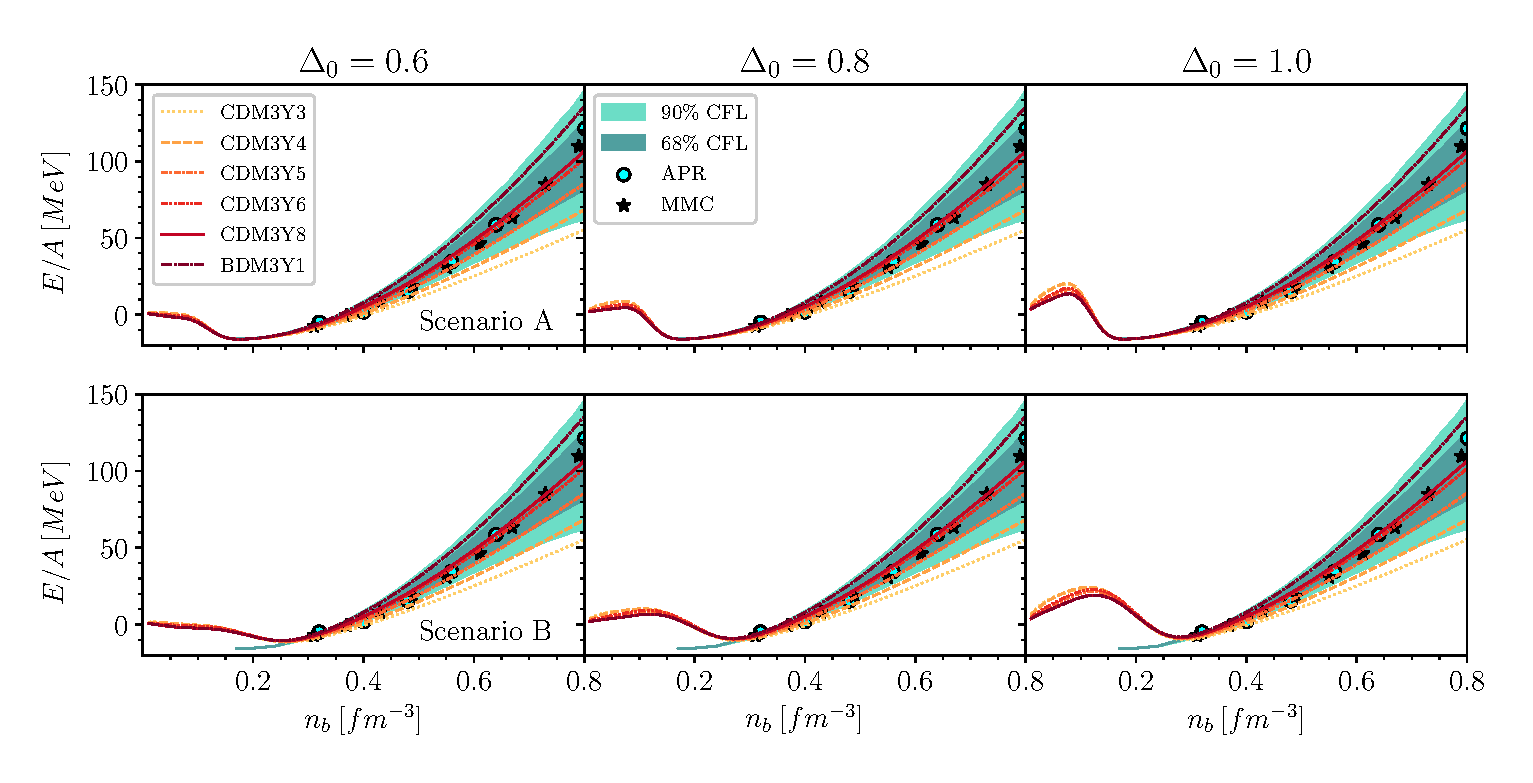
\includegraphics[width=\textwidth]{fig/EAS.eps}
    \caption{Same as Figure \ref{fig:s} for the energy per baryon $E/A$ of symmetric \gls{NM}.}
    \label{fig:eas}
\end{figure} 

On the other hand, the density-dependence of $S$ is also investigated through the symmetry coefficient $J$, slope parameter $L$ and curvature $K_{sym}$, which are taken by expanding the symmetry energy at saturation density $n_0$, i.e. \citep{tan2020spin,li2008recent,horowitz2014way,lattimer2014symmetry} 
\begin{equation}
    S(n_b, \Delta_n, \Delta_p) = J(\Delta_n, \Delta_p) + \frac{L(\Delta_n, \Delta_p)}{3} \left( \frac{n_b - n_0}{n_0} \right) + \frac{K_{sym}(\Delta_n, \Delta_p)}{18} \left( \frac{n_b - n_0}{n_0} \right)^2 + \ldots
    \label{eq:pars}
\end{equation}
as well as the nuclear incompressibility defined at saturation density
\begin{equation}
    K(\Delta_n, \Delta_p) = 9 \left.\pdv{P_b(n_b, \delta=0,\Delta_n,\Delta_p)}{n_b}\right|_{n_b \to n_0}
        \label{eq:K}
\end{equation}
with $P_b$ being the baryonic pressure.

Among these quantities, the incompressibility $K$ of symmetric \gls{NM} has been intensively studied the most in several structure studies of monopole excitations (e.g. \cite{garg2018compression}), \gls{HI} collisions and refractive \gls{NN} scattering \citep{khoa2007nuclear}. The \gls{HF} result in Table \ref{tab:pars} leaves only the case of $\Delta=0.0$ to satisfy the constrained value $K\approx 240^{+20}_{-20}\:MeV$ deduced from these studies, since in this case, $K$ ranges from $227-257\:MeV$, which is well within the empirical value. Apart from the nuclear incompressibility $K$, recently, the values of $J$, $L$, $K_{sym}$ are much more well determined from the study of \cite{essick2021astrophysical} by combining astrophysical data with PREX-II and chiral effective field theory, which yields $J\approx 34^{+3}_{-3}\:MeV$, $L\approx 58^{+19}_{-19}\:MeV$ and $K_{sym}\approx -107^{+128}_{-138}\:MeV$. The value of $J$ and $L$ obtained with \gls{HF} formalism (Table \ref{tab:pars}) remain well within the interval suggested by this study, except for when the polarization $\Delta$ approaches $\approx 1.0$. The curvature $K_{sym}$, however, has not been as well determined as the other quantities, therefore it still widely ranges for different scenarios and no further selection on the \gls{EoS} with it can be done.
\begin{table}[ht!]
    \centering
    \caption{The symmetry coefficient $J$, slope parameter $L$, curvature $K_{sym}$ of the symmetric energy \eqref{eq:pars} and incompressibility $K$ \eqref{eq:K} of symmetric \gls{NM}, calculated using 4 different \gls{NN} interactions.}
    \label{tab:pars}
    \begin{tabular}{|c|C|C|C|C|C|}
        \hline
        Interaction & \Delta & J & L & K_{sym} & K\\
        \hline
        \multirow{3}{*}{CDM3Y4} & 0.0 & 28.97 & 48.38 & -60.49 & 227.96\\
        \cline{2-6}
                                & 0.5 & 30.83 & 52.63 & -54.54 & 294.58\\
        \cline{2-6}
                                & 1.0 & 37.26 & 63.81 & -66.58 & 498.50\\
        \hline
        \multirow{3}{*}{CDM3Y5} & 0.0 & 28.92 & 48.36 & -49.61 & 241.25\\
        \cline{2-6}
                                & 0.5 & 30.78 & 51.42 & -43.60 & 316.30\\
        \cline{2-6}
                                & 1.0 & 37.20 & 59.37 & -47.54 & 545.96\\
        \hline
        \multirow{3}{*}{CDM3Y6} & 0.0 & 28.94 & 48.36 & -42.09 & 251.86\\
        \cline{2-6}
                                & 0.5 & 31.19 & 49.93 & -33.86 & 319.51\\
        \cline{2-6}
                                & 1.0 & 38.67 & 52.27 & -25.26 & 526.68\\
        \hline
        \multirow{3}{*}{CDM3Y8} & 0.0 & 28.95 & 48.39 & -28.65 & 257.13\\
        \cline{2-6}
                                & 0.5 & 31.35 & 49.58 & -21.86 & 343.25\\
        \cline{2-6}
                                & 1.0 & 39.23 & 50.53 & -16.40 & 602.65\\
        \hline
    \end{tabular}
\end{table}

\section{\textbeta-stable spin-polarized neutron star matter}%
\label{sec:textbeta_stable_spin_polarized_neutron_star_matter}

After the \gls{HF} calculation, we were able to obtain a numerical \gls{HF} energy density $\varepsilon_{HF}$. However, it is in fact impossible for a \gls{NS} to exist while consisting of purely nucleon. In order to compensate for this issue, leptons ($e^-$ and $\mu^-$) have to be introduced to the matter constituents and the $npe\mu$ matter has to satisfy the \emph{\textbeta-stable} condition \citep{glendenning2012compact}, i.e.
\begin{itemize}
        \item Charge balance
                \begin{equation}
                        n_p = n_e + n_\mu
                        \label{chargeEQ}
                \end{equation}
        \item Chemical potential balance
                \begin{equation}
                        \mu_n - \mu_p = \mu_e = \mu_\mu
                \end{equation}
                where $\mu_i = \pdv{\varepsilon}{n_i}$ ($i=n,p,e,\mu$) is the chemical potential of the $i$ particle.
\end{itemize}
The total energy density of the $npe\mu$ matter is thus
\begin{equation}
        \varepsilon = \varepsilon_{HF} + n_n m_n c^2 + n_p m_p c^2 + \varepsilon_e + \varepsilon_\mu 
\end{equation}
which leads to the nucleon chemical potential of the form
\begin{equation}
        \mu_\tau (n_n,n_p,\Delta_n,\Delta_p) = \frac{\partial \varepsilon}{\partial n_\tau}  = \frac{\partial \varepsilon_{HF}}{\partial n_\tau} + m_\tau c^2
\end{equation}
Let $\hat{\mu} = \mu_n - \mu_p$ be the leptons' chemical potential, \eqref{chargeEQ} is equivalent to\footnote{$\theta(x)$ is the Heaviside function, i.e. it returns $1$ for $x\geq 0$ and $0$ otherwise.}
\begin{equation}
        3\pi^2 (\hbar c)^3 n_p - \hat{\mu}^3 - \left[ \hat{\mu}^2 - (m_\mu c^2)^2 \right]^{3/2} \theta(\hat{\mu} - m_\mu c^2) = 0
\end{equation}
Note that only beyond the muon threshold density $\mu_e > m_\mu c^2 \approx 105.6\:MeV$ do muons appear in the system. Furthermore, under strong magnetic field like that of a magnetar, we can approximate $\Delta_n \approx -\Delta_p \approx \Delta$ and reduce the \gls{EoS} to depend on just the baryon polarization $\Delta$ alone, and the more baryon polarized, the stronger the magnetic field of the \gls{NS}.\par
For a fixed value of $\Delta$, we are able to obtain a density function of the form $n_n (n_b, \Delta)$ and $n_p (n_b, \Delta)$, which in turn gives the lepton chemical potential $\hat{\mu}(n_b,\Delta) = \hat{\mu}(n_n,n_p)$ On the other hand, the leptons' densities are then
\begin{equation}
        n_e(n_b,\Delta) = \frac{ \hat{\mu}^3(n_b,\Delta)}{ 3\pi^2 (\hbar c)^3} \quad\text{and}\quad n_\mu(n_b,\Delta) = \frac{ \Big[\hat{\mu}^2(n_b,\Delta) - (m_\mu c^2)^2\Big]^{3/2}}{ 3\pi^2 (\hbar c)^3} \theta(\hat{\mu}(n_b,\Delta)-m_\mu c^2)
\end{equation} 
Consider the $e^-$ and $\mu^-$ to be systems of relativistic Fermi gas, then their respective energy densities and pressure contributions are ($l=e,\mu$) \citep{moustakidis2009equation}
\begin{equation}
        \varepsilon_l(n_b,\Delta) = \frac{ 2}{ (2\pi)^3} \int_{{0}}^{{[3\pi^2n_l(n_b,\Delta)]^{1/3}}} {\sqrt{\hbar^2 c^2 k^2 + m_l^2 c^4}} \: d^3{\mathbf{k}}
\end{equation} 
and
\begin{equation}
        P_l(n_b,\Delta) = \frac{ 1}{ 3} \frac{ 2}{ (2\pi)^3} \int_{{0}}^{{[3\pi^2 n_l(n_b,\Delta)]^{1/3}}} { \frac{ \hbar^2 c^2 k^2}{ \sqrt{\hbar^2 c^2 k^2 + m_l^2 c^4}} } \: d^3{\mathbf{k}}
\end{equation} 
Plus, from the \gls{HF} study, the baryonic pressure is given by
\begin{equation}
    P_b = n_b^2 \pdv{}{n_b} \left[ \frac{E}{A}(n_b,\delta,\Delta) \right]
\end{equation}
Finally, we obtain the total energy density-dependence on baryon density as 
\begin{equation}
        \varepsilon(n_b,\Delta) = \varepsilon_{HF}(n_b,\Delta) + n_n(n_b,\Delta)m_n c^2 + n_p(n_b,\Delta)m_p c^2 + \varepsilon_e(n_b,\Delta) + \varepsilon_\mu(n_b,\Delta)
\end{equation}
and the total pressure of \gls{NS} matter
\begin{equation}
        P(n_b,\Delta) = P_b(n_b,\Delta) + P_e(n_b,\Delta) + P_\mu(n_b,\Delta)
\end{equation}
The mass-energy density of \gls{NS} matter is also defined as $\rho = \varepsilon/c^2$, which will be used as input for the \gls{TOV} equation in Chapter \ref{chap:ns_prop}.

In addition, the \gls{EoS} of the \gls{NS}'s crust (very low baryon density region with $n_b \lesssim 0.01\:fm^{-3}$) is adopted from the Compress Liquid Drop Model calculation \citep{douchin2000nuclear,douchin2001unified}, which was also shown by \cite{tan2020spin} that the magnetization of the crust has little effects on \gls{NS} properties. In Figure \ref{fig:p}, we show the total pressure of \gls{NS} matter $P(n_b)$ following the \gls{HF} calculation of 4 different versions of the density-dependent \gls{NN} interaction endowed with different levels of polarization. These results are simultaneously compared with the empirical pressure obtained from the ``spectral'' \gls{EoS} inferred from the Bayesian analysis of the GW170817 event \citep{abbott2018gw170817}. It is clear that the larger $K$ an interaction version has (Table \ref{tab:pars}), the more the generated \gls{NM} can be compressed to higher pressure at high density, and the model CDM3Y4 can be excluded since it is unlikely to satisfy the constraint derived by \cite{abbott2018gw170817}, while the other versions still lie inside of the 90\% \gls{CFL} region at $\Delta\approx 0.0$. In general, the pressures calculated by these 4 models follow well the empirical values from $\approx \rho_0$ to their corresponding maximum central density, i.e. the total pressure at twice and six times nuclear saturation density is within the range $P(2\rho_0)\approx 3.5^{+2.7}_{-1.7}\times 10^{34}$ and $P(6\rho_0)\approx 9.0^{+7.9}_{-2.6}\times 10^{35}\:dyn/cm^2$ at 90\% \gls{CFL}. Plus, at increasing spin polarization, the pressure tends to be stronger, indicated by a raise of $P(\rho_b)$ most significantly at the low density region. Taking all of the \gls{EoS} constraint up until now into account, the value suggested by the empirical study tends to favor models with higher $K$ value and smaller spin polarization.
\begin{figure}[ht!]
        \centering
        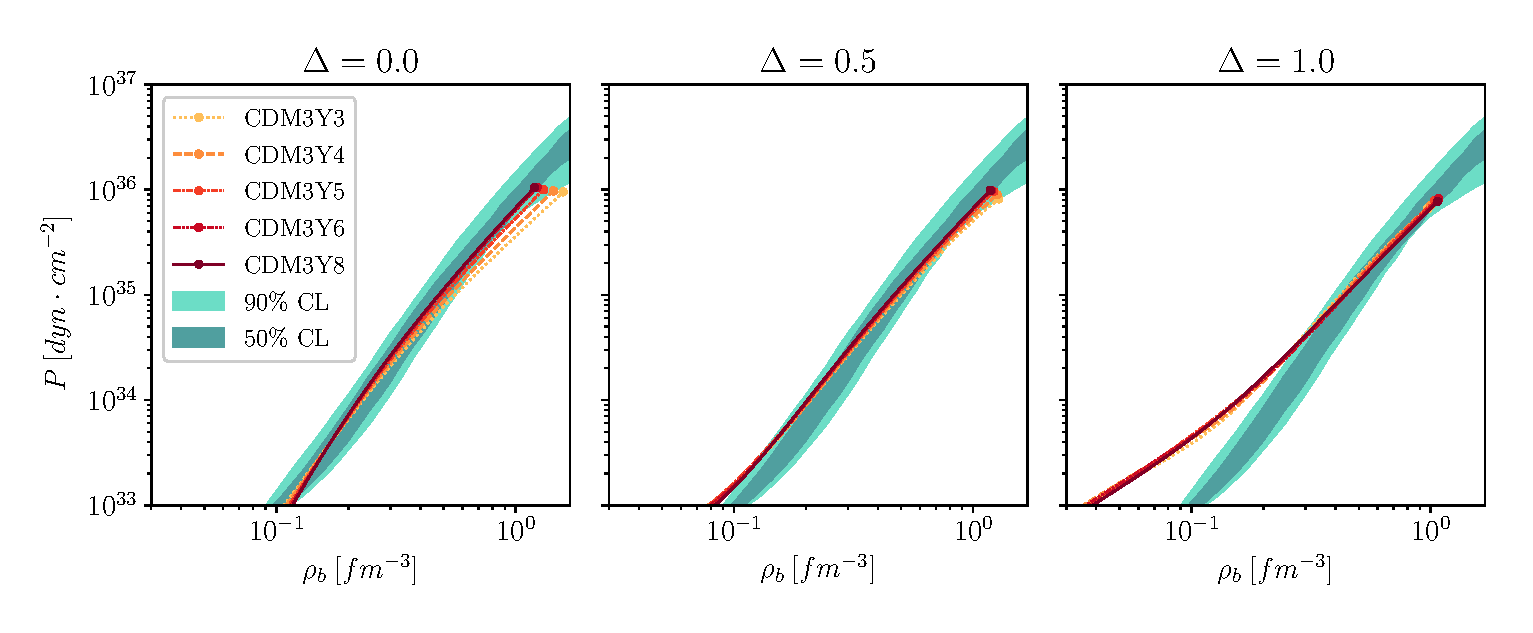
\includegraphics[width=\textwidth]{fig/P.eps}
        \caption{Same as Figure \ref{fig:s} for the pressure $P$ as a function of \emph{rest baryon mass density} $\rho_b$ along with empirical pressure given by the ``Spectral'' \gls{EoS} from the Bayesian analysis of the GW170817 data \citep{abbott2018gw170817} with 50\% (light gray) and 90\% (dark gray) confidence level. The dot at the end of each line corresponds to the central baryon density $n_b$ of maximum \gls{NS} mass.}
        \label{fig:p}
\end{figure} 
